\clearpage

\lehead[]{\normalfont\sffamily\hspace*{-2.00cm}\textcolor{white}{\colorbox{lightblue}{\parbox[c][0.70cm][b]{1.60cm}{
\makebox[1.60cm][r]{\thechapter}\\ \makebox[1.60cm][r]{ÜBUNG}}}}\hspace{0.17cm}\textcolor{lightblue}{\chaptertitle}}
\rohead[]{\textcolor{lightblue}{\chaptertitle}\normalfont\sffamily\hspace*{0.17cm}\textcolor{white}{\colorbox{lightblue}{\parbox[c][0.70cm][b]{1.60cm}{\thechapter\\
ÜBUNG}}}\hspace{-2.00cm}}
%\chead[]{}
\rehead[]{\textcolor{lightblue}{AvHG, Inf, My}}
\lohead[]{\textcolor{lightblue}{AvHG, Inf, My}}

\section{ER-Modell -- Übung}

\subsection{Aufgabe 1: Interpretation eines ER-Diagramms \tagPflicht}
\noindent \emph{Schwerpunkt: ER-Diagramme lesen (Entitätstypen, Attribute, Primärschlüssel und Kardinalitäten interpretieren).}

\begin{compactenum}[a)]
\item Interpretiere das folgende Entity-Relationship-Diagramm:

\vspace{2mm}
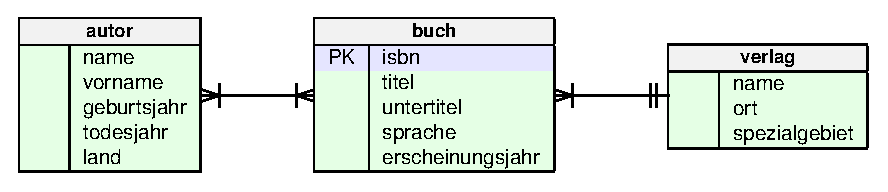
\includegraphics[width=0.80\textwidth]{./inf/SEKII/34_Datenbanken_und_ER-Modell/ermAufgabe1.eps}
\vspace{2mm}

Achtung: Das abgebildete ER-Diagramm ist unvollständig. Es fehlen -- unter
anderem -- einige Schlüsselfelder! Welche?

Vervollständige das ER-Diagramm!

\vspace{1mm}

\item Erstelle ein SQL-Skript \myFile{buecherei.sql}, mit dem diese
Datenbank erzeugt werden kann (diesen Aufgabenteil kannst du im Anschluss an das
nächste Kapitel zu SQL bearbeiten).
\end{compactenum}


\subsection{Aufgabe 2: Kardinalitäten \tagPflicht}
\noindent \emph{Schwerpunkt: Festigung der Beziehungstypen ($1:1$, $1:n$, $n:m$) an praktischen Beispielen.}

Welche Art von Beziehung besteht zwischen folgenden Entitätstypen? 

\emph{Achtung}: Entitätstyp (also Tabelle) bedeutet natürlich auch, dass es
jeweils mehrere Entitäten (Datensätze) gibt -- von beiden genannten
Entitätstypen existieren also jeweils mehrere Einträge in der Datenbank!

\begin{compactenum}[a)]
\item Mann, Frau (Beziehung: \glqq verheiratet\grqq )
\item Lehrer, Schüler
\item Esstisch, Stuhl
\item Tutor, Tutand
\item Schauspieler, Kinofilm (Beziehung: \glqq spielen in\grqq )
\end{compactenum}


\subsection{Aufgabe 3: Datenbankentwurf \tagZusatz \tagLK}
\noindent \emph{Schwerpunkt: Eigenständige Entwicklung eines Entity-Relationship-Diagramms aus einer verbalen Problembeschreibung.}

\begin{compactenum}[a)] 
\item Entwirf ein ER-Diagramm für einen Videoverleih:\\
Für die Videos sollen der Titel, der Regisseur, das Erscheinungsjahr und eine
Identifikationsnummer abgespeichert werden. Für jeden Kunden wird die
vollständige Adresse abgespeichert. Ein Video darf maximal zwei Wochen
ausgeliehen werden. Danach ist eine einmalige Verlängerung um weitere zwei
Wochen möglich. Es ist wichtig, dass die Informationen über die Ausleihe nach
Rückgabe eines Videos nicht gelöscht werden, damit man im Nachhinein überprüfen
kann, wer wann welches Video ausgeliehen hatte.
\item Erstelle ein SQL-Skript \myFile{videothek.sql}, mit dem diese
Datenbank erzeugt werden kann (ebenfalls im Anschluss an das nächste Kapitel).
\end{compactenum}

\pagebreak
 
\subsection{Aufgabe 4: Vergleich mit UML \tagLK}
\noindent \emph{Schwerpunkt: Abgrenzung zwischen Datenmodellierung (ER-Modell) und objektorientierter Modellierung (UML-Klassendiagramm).}

Vergleiche das Entity-Relationship-Modell mit dem Modell objektorientierter
Programmiersachen, die man mit UML-Diagrammen entwirft.


\begin{compactenum}[a)]
\item Setze die Begriffe aus UML mit dem ER-Modell in Beziehung:

\vspace{2mm}

\bgroup
\def\arraystretch{1.2}
\begin{tabular}{|l|l|}\hline
\textbf{Begriff in UML} & \textbf{Entsprender Begriff im ER-Modell\hspace{2cm}}
\\
\hline Klasse & \\ \hline
Objekt & \\ \hline
Attribut & \\ \hline
Methode & \\ \hline
(normale) Beziehung & \\ \hline
Aggregationsbeziehung & \\ \hline
Vererbungsbeziehung & \\ \hline
\end{tabular}
\egroup

\vspace{2mm}

\item Was sind die wesentlichen Unterschiede zwischen dem ER-Modell und dem
UML-Modell?
\end{compactenum}
